% Options for packages loaded elsewhere
\PassOptionsToPackage{unicode}{hyperref}
\PassOptionsToPackage{hyphens}{url}
\PassOptionsToPackage{dvipsnames,svgnames,x11names}{xcolor}
%
\documentclass[
  letterpaper,
  DIV=11,
  numbers=noendperiod]{scrartcl}

\usepackage{amsmath,amssymb}
\usepackage{iftex}
\ifPDFTeX
  \usepackage[T1]{fontenc}
  \usepackage[utf8]{inputenc}
  \usepackage{textcomp} % provide euro and other symbols
\else % if luatex or xetex
  \usepackage{unicode-math}
  \defaultfontfeatures{Scale=MatchLowercase}
  \defaultfontfeatures[\rmfamily]{Ligatures=TeX,Scale=1}
\fi
\usepackage{lmodern}
\ifPDFTeX\else  
    % xetex/luatex font selection
\fi
% Use upquote if available, for straight quotes in verbatim environments
\IfFileExists{upquote.sty}{\usepackage{upquote}}{}
\IfFileExists{microtype.sty}{% use microtype if available
  \usepackage[]{microtype}
  \UseMicrotypeSet[protrusion]{basicmath} % disable protrusion for tt fonts
}{}
\makeatletter
\@ifundefined{KOMAClassName}{% if non-KOMA class
  \IfFileExists{parskip.sty}{%
    \usepackage{parskip}
  }{% else
    \setlength{\parindent}{0pt}
    \setlength{\parskip}{6pt plus 2pt minus 1pt}}
}{% if KOMA class
  \KOMAoptions{parskip=half}}
\makeatother
\usepackage{xcolor}
\setlength{\emergencystretch}{3em} % prevent overfull lines
\setcounter{secnumdepth}{-\maxdimen} % remove section numbering
% Make \paragraph and \subparagraph free-standing
\ifx\paragraph\undefined\else
  \let\oldparagraph\paragraph
  \renewcommand{\paragraph}[1]{\oldparagraph{#1}\mbox{}}
\fi
\ifx\subparagraph\undefined\else
  \let\oldsubparagraph\subparagraph
  \renewcommand{\subparagraph}[1]{\oldsubparagraph{#1}\mbox{}}
\fi


\providecommand{\tightlist}{%
  \setlength{\itemsep}{0pt}\setlength{\parskip}{0pt}}\usepackage{longtable,booktabs,array}
\usepackage{calc} % for calculating minipage widths
% Correct order of tables after \paragraph or \subparagraph
\usepackage{etoolbox}
\makeatletter
\patchcmd\longtable{\par}{\if@noskipsec\mbox{}\fi\par}{}{}
\makeatother
% Allow footnotes in longtable head/foot
\IfFileExists{footnotehyper.sty}{\usepackage{footnotehyper}}{\usepackage{footnote}}
\makesavenoteenv{longtable}
\usepackage{graphicx}
\makeatletter
\def\maxwidth{\ifdim\Gin@nat@width>\linewidth\linewidth\else\Gin@nat@width\fi}
\def\maxheight{\ifdim\Gin@nat@height>\textheight\textheight\else\Gin@nat@height\fi}
\makeatother
% Scale images if necessary, so that they will not overflow the page
% margins by default, and it is still possible to overwrite the defaults
% using explicit options in \includegraphics[width, height, ...]{}
\setkeys{Gin}{width=\maxwidth,height=\maxheight,keepaspectratio}
% Set default figure placement to htbp
\makeatletter
\def\fps@figure{htbp}
\makeatother

\KOMAoption{captions}{tableheading}
\makeatletter
\@ifpackageloaded{caption}{}{\usepackage{caption}}
\AtBeginDocument{%
\ifdefined\contentsname
  \renewcommand*\contentsname{Table of contents}
\else
  \newcommand\contentsname{Table of contents}
\fi
\ifdefined\listfigurename
  \renewcommand*\listfigurename{List of Figures}
\else
  \newcommand\listfigurename{List of Figures}
\fi
\ifdefined\listtablename
  \renewcommand*\listtablename{List of Tables}
\else
  \newcommand\listtablename{List of Tables}
\fi
\ifdefined\figurename
  \renewcommand*\figurename{Figure}
\else
  \newcommand\figurename{Figure}
\fi
\ifdefined\tablename
  \renewcommand*\tablename{Table}
\else
  \newcommand\tablename{Table}
\fi
}
\@ifpackageloaded{float}{}{\usepackage{float}}
\floatstyle{ruled}
\@ifundefined{c@chapter}{\newfloat{codelisting}{h}{lop}}{\newfloat{codelisting}{h}{lop}[chapter]}
\floatname{codelisting}{Listing}
\newcommand*\listoflistings{\listof{codelisting}{List of Listings}}
\makeatother
\makeatletter
\makeatother
\makeatletter
\@ifpackageloaded{caption}{}{\usepackage{caption}}
\@ifpackageloaded{subcaption}{}{\usepackage{subcaption}}
\makeatother
\ifLuaTeX
  \usepackage{selnolig}  % disable illegal ligatures
\fi
\usepackage{bookmark}

\IfFileExists{xurl.sty}{\usepackage{xurl}}{} % add URL line breaks if available
\urlstyle{same} % disable monospaced font for URLs
\hypersetup{
  pdftitle={SUPREMA FL - REFERENCIAL DE MANEJO AGRONÓMICO},
  pdfauthor={Tecnología y Desarrollo de Aproscello},
  colorlinks=true,
  linkcolor={blue},
  filecolor={Maroon},
  citecolor={Blue},
  urlcolor={Blue},
  pdfcreator={LaTeX via pandoc}}

\title{SUPREMA FL - REFERENCIAL DE MANEJO AGRONÓMICO}
\usepackage{etoolbox}
\makeatletter
\providecommand{\subtitle}[1]{% add subtitle to \maketitle
  \apptocmd{\@title}{\par {\large #1 \par}}{}{}
}
\makeatother
\subtitle{Otra de nuestras nuevas variedades de arroz para Venezuela}
\author{Tecnología y Desarrollo de Aproscello}
\date{2024-12-11}

\begin{document}
\maketitle

\renewcommand*\contentsname{Table of contents}
{
\hypersetup{linkcolor=}
\setcounter{tocdepth}{3}
\tableofcontents
}
\begin{figure}[H]

{\centering 
\includegraphics[width=1.27083in,height=0.72917in]{logo.png}

}

\caption{Rif: J-08507040-0}

\end{figure}%

\subsection{SUPREMA FL}\label{suprema-fl}

SUPREMA FL es otra de nuestras nuevas variedades de arroz que junto a la
\textbf{RESILIA FL} le presentamos a todos los productores de arroz de
Venezuela. Una vez cumplidos todos los requisitos establecidos por la
\textbf{\emph{Comisión Nacional de Semilla}} (CONASEM), le fue asignado
el \textbf{\emph{código Nº CNS-CC-22-502-12}} en el
\textbf{\emph{Registro Nacional de Cultivares Comerciales}}.

La variedad \textbf{\emph{SUPREMA FL}}, proviene del cruce de
FL05512-7P-6-1P/FL02066-4P-1-1P-2P-M-1P-M-M-M-F11//FL04574-1P-4-3P-1P-M
y tiene por \emph{Pedigree FL08310-4P-1-3P-3P-M-2PY-M}.

Fue obtenida en el \textbf{\emph{Fondo Latinoamericano de Arroz de
Riego}} (FLAR) durante las generaciones segregantes F2 a F5; luego fue
seleccionada y desarrollada por el programa de mejoramiento de la
\textbf{\emph{Asociación de Productores de Semilla Certificada de los
Llanos Occidentales}} (APROSCELLO) con el apoyo de la
\textbf{\emph{Fundación Nacional del Arroz}} (FUNDARROZ).

\begin{figure}[H]

{\centering 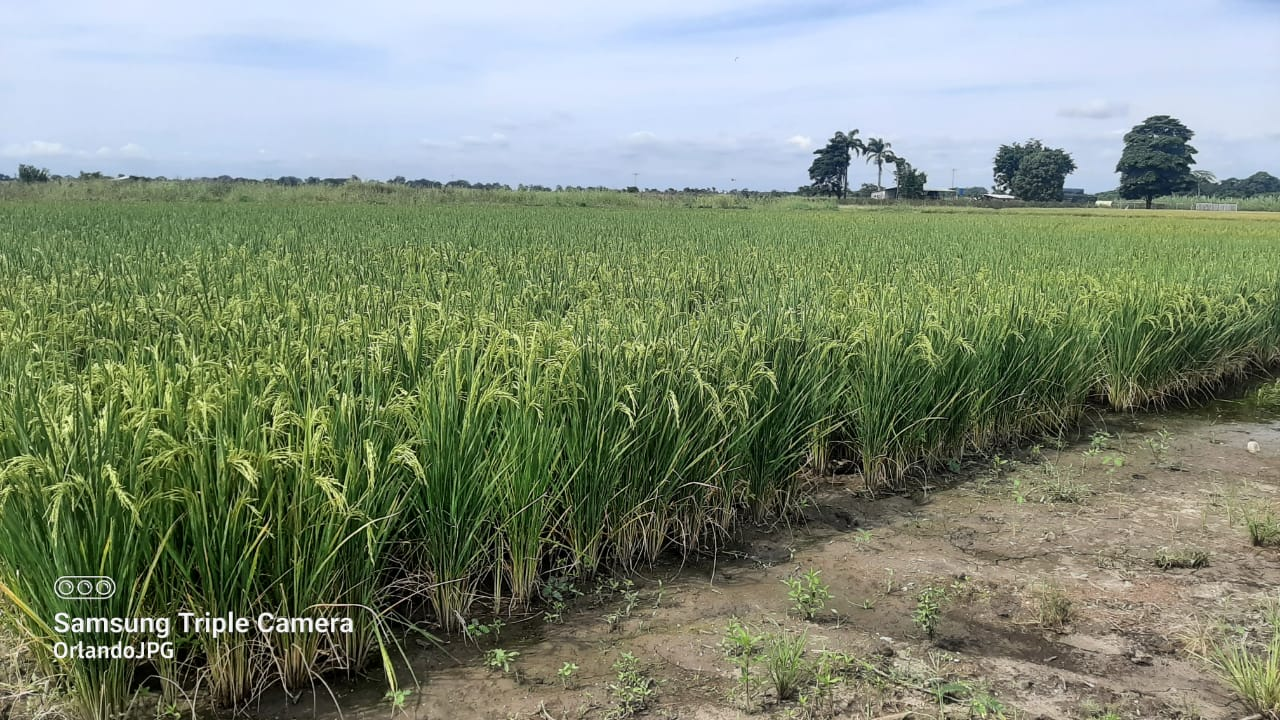
\includegraphics{AP009-8.jpeg}

}

\caption{Suprema FL, durante la fase de desarrollo de variedades}

\end{figure}%

\subsubsection{\texorpdfstring{\textbf{Características
agronómicas}}{Características agronómicas}}\label{caracteruxedsticas-agronuxf3micas}

\begin{longtable}[]{@{}lc@{}}
\toprule\noalign{}
\endhead
\bottomrule\noalign{}
\endlastfoot
Altura de la planta (cm) & 98 - 105 \\
Ciclo & Intermedio (115-120 días) \\
Hábito de crecimiento & Semi-compacto \\
Macollamiento & Buena capacidad \\
Color de la hoja & Verde \\
Reacción al desgrane & Moderadamente difícil \\
Reacción al volcamiento & Resistente \\
Tallo & Fuerte y flexible \\
Fertilidad (\%) & 90.58 - 97.51 \\
Nº de Granos por panícula & 176 - 237 \\
Longitud de la panícula (cm) & 23.5 - 32.1 \\
Retraso a cosecha & Resistente \\
Potencial de rendimiento (TN/ha) & Superior a 8,5 \\
\end{longtable}

\subsubsection{\texorpdfstring{\textbf{Reacción a plagas y
enfermedades}}{Reacción a plagas y enfermedades}}\label{reacciuxf3n-a-plagas-y-enfermedades}

\begin{longtable}[]{@{}lc@{}}
\toprule\noalign{}
\endhead
\bottomrule\noalign{}
\endlastfoot
Piricularia hoja (\emph{Pyricularia oryzae} ) & 0 - 3 \\
Piricularia cuello (\emph{Pyricularia oryzae} ) & 0 - 3 \\
Helminthosporiosis en hoja (\emph{Helminthosporium oryzae}) & 0 - 3 \\
Helminthosporiosis en cuello (\emph{Helminthosporium oryzae}) & 0 - 3 \\
Escaldado (\emph{Rhynchosporium oryzae}) & 0 - 3 \\
Manchado del grano & 0 - 3 \\
Virus Hoja Blanca & 0 - 5 \\
Sogata (\emph{Tagosodes orizicolus}) & 0 - 3 \\
\end{longtable}

\begin{itemize}
\item
  La escala de medición va desde 0 a 9.

  \begin{itemize}
  \item
    0 significa que no presentó síntomas y es resistente.
  \item
    9 es altamente susceptible.
  \end{itemize}
\end{itemize}

\subsubsection{\texorpdfstring{\textbf{Características de la
semilla}}{Características de la semilla}}\label{caracteruxedsticas-de-la-semilla}

\begin{longtable}[]{@{}lc@{}}
\caption{Características de la semilla}\tabularnewline
\toprule\noalign{}
\endfirsthead
\endhead
\bottomrule\noalign{}
\endlastfoot
Longitud mm) & 9.0 - 11.0 \\
Ancho (mm) & 2.0 - 3.0 \\
Espesor (mm) & 2.0 \\
Arista & Ausente \\
Peso de 1000 semillas (gr) & 24.0 - 28.0 \\
\end{longtable}

\subsection{\texorpdfstring{\textbf{REFERENCIAL DE MANEJO
AGRONÓMICO}}{REFERENCIAL DE MANEJO AGRONÓMICO}}\label{referencial-de-manejo-agronuxf3mico}

El \emph{Referencial de Manejo Agronómico de la variedad \textbf{SUPREMA
FL}} constituye una guía imprescindible para garantizar la optimización
de su manejo en campo y ayudará a que el productor alcance altos
rendimientos. Recomendamos que tanto agrotécnicos como los productores
estudien con detenimiento cada una de estas recomendaciones que aun
cuando son de carácter general, resultan suficientes como base
orientativa para la toma de decisiones en cada fase de desarrollo del
cultivo.

\subsubsection{\texorpdfstring{\textbf{Densidad de
siembra}}{Densidad de siembra}}\label{densidad-de-siembra}

En nuestras evaluaciones experimentales y semicomerciales se determinó
que la SUPREMA FL puede ser manejada bajo diferentes densidades de
siembra, sin embargo, para definir la cantidad de semilla por hectárea
recomendamos sopesar la modalidad de siembra a implementar; a
continuación hacemos las consideraciones pertinentes para cada sistema.

\paragraph{\texorpdfstring{\textbf{\emph{Sistema de barro batido y
semilla
pregerminada}}}{Sistema de barro batido y semilla pregerminada}}\label{sistema-de-barro-batido-y-semilla-pregerminada}

Al igual que otras variedades comerciales, recomendamos que el
pregerminado se realice dándole una primera fase de remojo que puede
durar entre 24 a 36 horas y durante una segunda fase, luego de sacar la
semilla del agua colocar la semilla bajo sombra durante un tiempo no
menor de 24 horas y no mayor de 28 horas, al finalizar esta segunda
fase, la semilla estará lista la siembra. Consideramos que el productor
maneje densidades de entre 90 y 120 kg/ha de semilla certificada. A
nivel comercial le damos preferencia a usar 100 kg/ha.

\paragraph{\texorpdfstring{\textbf{\emph{Sistemas de labranza en suelo
seco y otros
alternativos}}}{Sistemas de labranza en suelo seco y otros alternativos}}\label{sistemas-de-labranza-en-suelo-seco-y-otros-alternativos}

En sistemas de labranza reducida o conservacionista, recomendamos
densidades de entre los 60 y 90 kg/ha de semilla certificada; algunas
consideraciones importantes son las siguientes:

\begin{itemize}
\item
  Profundidad de siembra en 2,5 cm de promedio y que ésta no sea mayor a
  3 cm.
\item
  Si la siembra es bajo el esquema de semilla tapada con rastra de tiro,
  se recomendamos incrementar entre un 5 \% a 7 \% la densidad con el
  propósito de compensar la pérdida por las semillas que queden muy
  profunda y no son capaces de emerger.
\end{itemize}

\begin{figure}[H]

{\centering 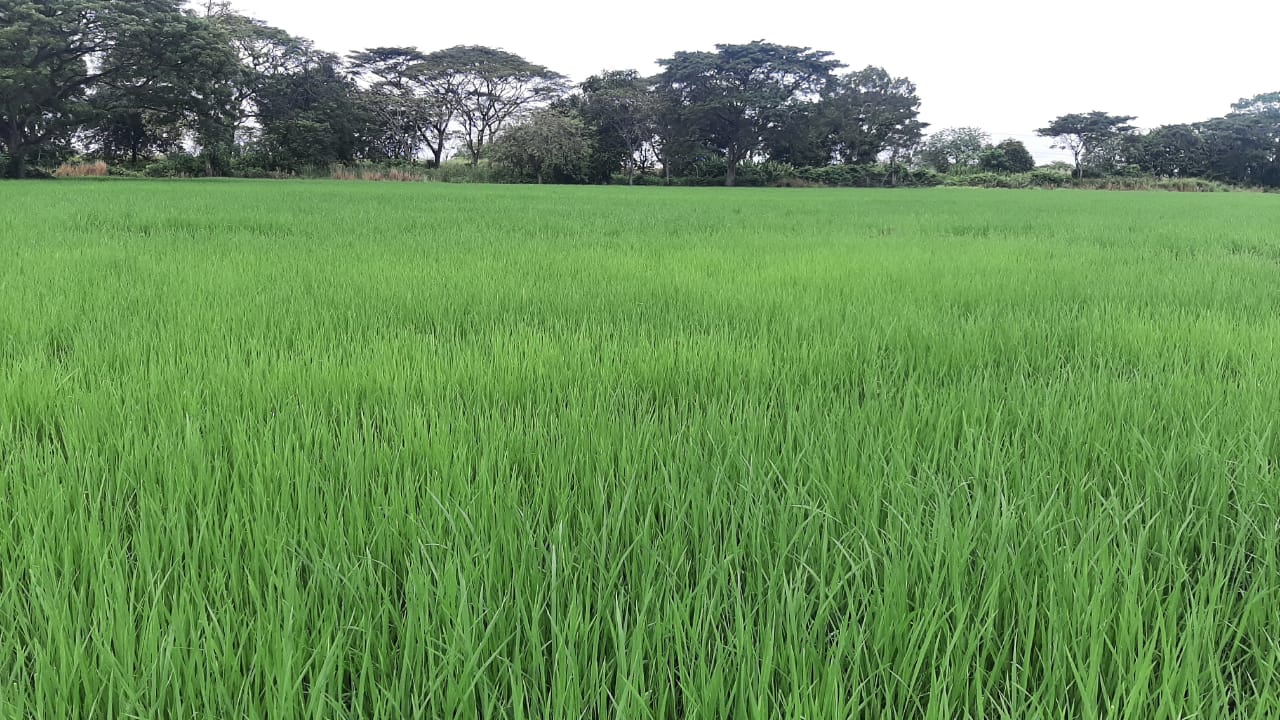
\includegraphics{AP009-5.jpeg}

}

\caption{Suprema FL, sembrada a 80 kg/ha}

\end{figure}%

\subsubsection{\texorpdfstring{\textbf{Control de
malezas}}{Control de malezas}}\label{control-de-malezas}

Como componente fundamental del manejo integral del cultivo hemos
sometido a evaluación el comportamiento de la SUPREMA FL frente a las
principales moléculas de herbicidas que se utilizan en el cultivo de
arroz utilizando las dosis recomendadas utilizando los productos solos y
en mezclas tradicionales. Durante la implementación de las pruebas se
realizaron aplicaciones en condiciones de ambiente controlado, así como
en parcelas semicomerciales para validar en condiciones de campo, se
consideraron testigos absolutos y mezclas tradicionales de herbicidas
con preemergentes, postemergentes, de contacto y sistémicos. Como
resultado se pudo observar que la variedad \textbf{\emph{SUPREMA FL}}
mostró excelente comportamiento, no mostró ningún problemas de
fitotoxicidad y desarrollo normal del cultivo.

A continuación algunos tips de importancia en el control de malezas con
herbicidas:

\begin{itemize}
\item
  Cuando se utilice semilla pregerminada, se recomienda que los
  controles de malezas se realicen en pre-emergencia temprana, esto es,
  entre los 5 y 10 dds (días después de la siembra).
\item
  En el caso de usar semilla seca (no pregerminada) es completamente
  viable realizar aplicaciones de control de malezas entre los primeros
  3 días antes de la emergencia; sin embargo, es importante que la
  decisión sea avalada por un técnico que verifique el estado de avance
  de la etapa de germinación para no salirse del momento óptimo de
  aplicación.
\item
  Recuerde en mezcla donde esté presente propaniles no deben agregarse o
  mezclarse insecticidas fosforados o carbamatos.
\end{itemize}

\subsubsection{\texorpdfstring{\textbf{Manejo de la
fertilización}}{Manejo de la fertilización}}\label{manejo-de-la-fertilizaciuxf3n}

La fertilización es unas de las labores más importantes debido que está
asociada al óptimo desarrollo del cultivo y la mayor expresión del
potencial de rendimiento del cultivo de arroz. Durante la etapa de
desarrollo de la variedad SUPREMA FL, nos esforzamos en obtener el
patrón de extracción de nitrógeno, fósforo y potasio por vía indirecta.

Recomendamos no improvisar en el diseño y la aplicación del plan de
fertilización a fin de garantizar la mejor nutrición posible y
garantizar el uso eficiente de los fertilizante. La base para armar el
plan es partir de un análisis de suelo que permita conocer la realidad
del suelo en cuanto a sus propiedades físico-químicas, así mismo
considerar la interacción entre la fecha de aplicación (momento
oportuno), el tipo de nutriente o elemento a aplicar y las dosis.

Nos atrevemos a proponer una plan de fertilización de referencia tomando
en cuenta los resultados de los ensayos realizados en cada zona y la
demanda específica de la variedad. sin embargo, no olvide realizar una
análisis riguroso de la información para ajustar los requerimientos.

\textbf{Tabla base para estimar necesidades nutricionales de la
variedad}

\begin{longtable}[]{@{}lc@{}}
\toprule\noalign{}
Elemento & Cantidad kg/ha \\
\midrule\noalign{}
\endhead
\bottomrule\noalign{}
\endlastfoot
Nitrógeno (N) & 160 a 180 \\
Fósforo (P\textsubscript{2}O\textsubscript{5}) & 25 a 31 \\
Potasio (K\textsubscript{2}O) & 115 a 122 \\
\end{longtable}

\textbf{1ra. Propuesta de fertilización con fósforo y potasio
incorporados y dos reabonos}

\begin{longtable}[]{@{}
  >{\raggedright\arraybackslash}p{(\columnwidth - 6\tabcolsep) * \real{0.4512}}
  >{\raggedright\arraybackslash}p{(\columnwidth - 6\tabcolsep) * \real{0.2439}}
  >{\raggedright\arraybackslash}p{(\columnwidth - 6\tabcolsep) * \real{0.1829}}
  >{\raggedright\arraybackslash}p{(\columnwidth - 6\tabcolsep) * \real{0.1220}}@{}}
\caption{dds = días después de la siembra; dde = días después de la
emergencia}\tabularnewline
\toprule\noalign{}
\begin{minipage}[b]{\linewidth}\raggedright
Momento
\end{minipage} & \begin{minipage}[b]{\linewidth}\raggedright
Fuente
\end{minipage} & \begin{minipage}[b]{\linewidth}\raggedright
Elementos
\end{minipage} & \begin{minipage}[b]{\linewidth}\raggedright
Cantidad
\end{minipage} \\
\midrule\noalign{}
\endfirsthead
\toprule\noalign{}
\begin{minipage}[b]{\linewidth}\raggedright
Momento
\end{minipage} & \begin{minipage}[b]{\linewidth}\raggedright
Fuente
\end{minipage} & \begin{minipage}[b]{\linewidth}\raggedright
Elementos
\end{minipage} & \begin{minipage}[b]{\linewidth}\raggedright
Cantidad
\end{minipage} \\
\midrule\noalign{}
\endhead
\bottomrule\noalign{}
\endlastfoot
Presiembra incorporado & Fósfoto diamónico & Fósforo (P) & Todo \\
Presiembra incorporado & Cloruro de potasio & Potasio (K) & Todo \\
Reabono entre los 16 a 20 dds o dde & Urea & Nitrógeno (N) & 60\% \\
Reabono entre los 40 a 45 dds o dde & Urea & Nitrógeno (N) & 40\% \\
\end{longtable}

\textbf{2da. Propuesta de fertilización en base a modalidad tradicional}

\begin{longtable}[]{@{}
  >{\raggedright\arraybackslash}p{(\columnwidth - 6\tabcolsep) * \real{0.4512}}
  >{\raggedright\arraybackslash}p{(\columnwidth - 6\tabcolsep) * \real{0.2439}}
  >{\raggedright\arraybackslash}p{(\columnwidth - 6\tabcolsep) * \real{0.1829}}
  >{\raggedright\arraybackslash}p{(\columnwidth - 6\tabcolsep) * \real{0.1220}}@{}}
\caption{dds = días después de la siembra; dde = días después de la
emergencia}\tabularnewline
\toprule\noalign{}
\begin{minipage}[b]{\linewidth}\raggedright
Momento
\end{minipage} & \begin{minipage}[b]{\linewidth}\raggedright
Fuente
\end{minipage} & \begin{minipage}[b]{\linewidth}\raggedright
Elementos
\end{minipage} & \begin{minipage}[b]{\linewidth}\raggedright
Cantidad
\end{minipage} \\
\midrule\noalign{}
\endfirsthead
\toprule\noalign{}
\begin{minipage}[b]{\linewidth}\raggedright
Momento
\end{minipage} & \begin{minipage}[b]{\linewidth}\raggedright
Fuente
\end{minipage} & \begin{minipage}[b]{\linewidth}\raggedright
Elementos
\end{minipage} & \begin{minipage}[b]{\linewidth}\raggedright
Cantidad
\end{minipage} \\
\midrule\noalign{}
\endhead
\bottomrule\noalign{}
\endlastfoot
Básica entre los 25 a 30 dds o dde & Fórmula completa & Nitrógeno (N) &
20\% \\
& & Fósforo (P) & Todo \\
& & Potasio (P) & 20\% \\
Reabono entre los 25 a 32 dds o dde & Urea & Nitrógeno (N) & 45\% \\
& Cloruro de potasio & Potasio (K) & 80\% \\
Reabono a los 45 dds o dde & Urea & Nitrógeno (N) & 40\% \\
\end{longtable}

Las cantidades de fertilizante expresadas en porcentaje (\%) del total
respectivo, no es una camisa de fuerza, sin embargo, debe usarse
cantidades que se acerquen a esos valores, entendiendo que todo va a
depender del total requerido por nutriente y la proporción del mismo
presente en la fuente utilizada.

Es importante resaltar que consideramos válido que si por razones de
logística la última enmienda de \textbf{\emph{nitrógeno}} no se pudiera
aplicar antes de la etapa de elongación, se recomienda esperar que esta
etapa termine para poder realizarla, esto evitará que la planta crezca
en altura por encima de su promedio lo que induciría a condiciones
favorables para el acame o vuelco. igual consideración debe tenerse en
caso que el técnico recomiende suplir un adicional de nitrógeno.

A continuación agregamos información complementaria sobre la
fertilización:

\begin{itemize}
\item
  \textbf{Nitrógeno (N):} No aplicar menos de 160 unidades/ha; no perder
  de vista la relación 1:1 con el potasio (K).
\item
  \textbf{Fósforo (P):} el cultivar mostró que para alcanzar un
  rendimiento superior a las 8 toneladas/ha, requirió la absorción de 31
  kg/ha de P\textsubscript{2}O\textsubscript{5}, en base a esta
  información se recomienda un promedio de 22 unidades/ha de
  P\textsubscript{2}O\textsubscript{5}, sin embargo, esta cantidad debe
  ser ajustada en función de la disponibilidad del elemento en el suelo.
\item
  \textbf{Potasio (K):} este elemento está relacinado con la sanidad
  integral del cultivar, la producción de materia seca y su potencial de
  rendimiento. El patrón de extracción determinado indirectamente mostró
  que las mejores respuestas en rendimiento de grano se alcanzaron con
  enmiendas de entre los 115 y 122 kg/ha de K\textsubscript{2}O;
  resaltamos que se pondere su aplicación en base al análisis de suelo y
  la dinámica del elemento en su relación con el nitrógeno (N) y el
  magnesio (Mg).
\item
  \textbf{Calcio, Magnesio y Azufre:} estos tres elementos juegan un
  importante papel dentro del desarrollo del cultivo y es importante
  considerar su enmienda para garantizar su equilibrio. Sin embargo,
  debemos que señalar que no ha sido posible determinar sus patrones de
  extracción, por lo que lo recomendado a continuación se basa en
  referencias de otros trabajos similares en arroz.

  \begin{itemize}
  \item
    Calcio: entre 11 y 16 kg/ha de Ca, preferiblemente con la
    fertilización básica.
  \item
    Magnesio: entre 8 y 12 kg/ha de Mg en la fertilización básica o en
    el primer reabono.
  \item
    Azufre: 16 y 22 kg/ha de S; preferiblemente en el primer reabono.
  \end{itemize}
\end{itemize}

\subsubsection{\texorpdfstring{\textbf{Manejo de
enfermedades}}{Manejo de enfermedades}}\label{manejo-de-enfermedades}

La variedad \textbf{\emph{SUPREMA FL}} fue evaluada con el rigor
necesario en diferentes ambientes para conocer su comportamiento frente
a las enfermedades fungosas más importantes del país (ver el apartado
\emph{Reacción frente a plagas y enfermedades)}. Aun cuando su desempeño
fue muy bueno frente a los patógenos más importantes, es necesario tener
presente que ante las variaciones climáticas que se están presentando en
los últimos años hay que estar atentos a las diferentes síntomas que se
puedan presentar y recomendamos que durante los meses del año donde se
registran constantes precipitaciones y altas temperaturas, se realicen
protecciones preventivas dirigidas a garantizar la sanidad integral de
cultivo y la panículabajo asesoría técnica, de esta manera se evitaría
posibles brotes del complejo de patógenos responsable del manchado de
granos.

\begin{figure}

\begin{minipage}{0.50\linewidth}

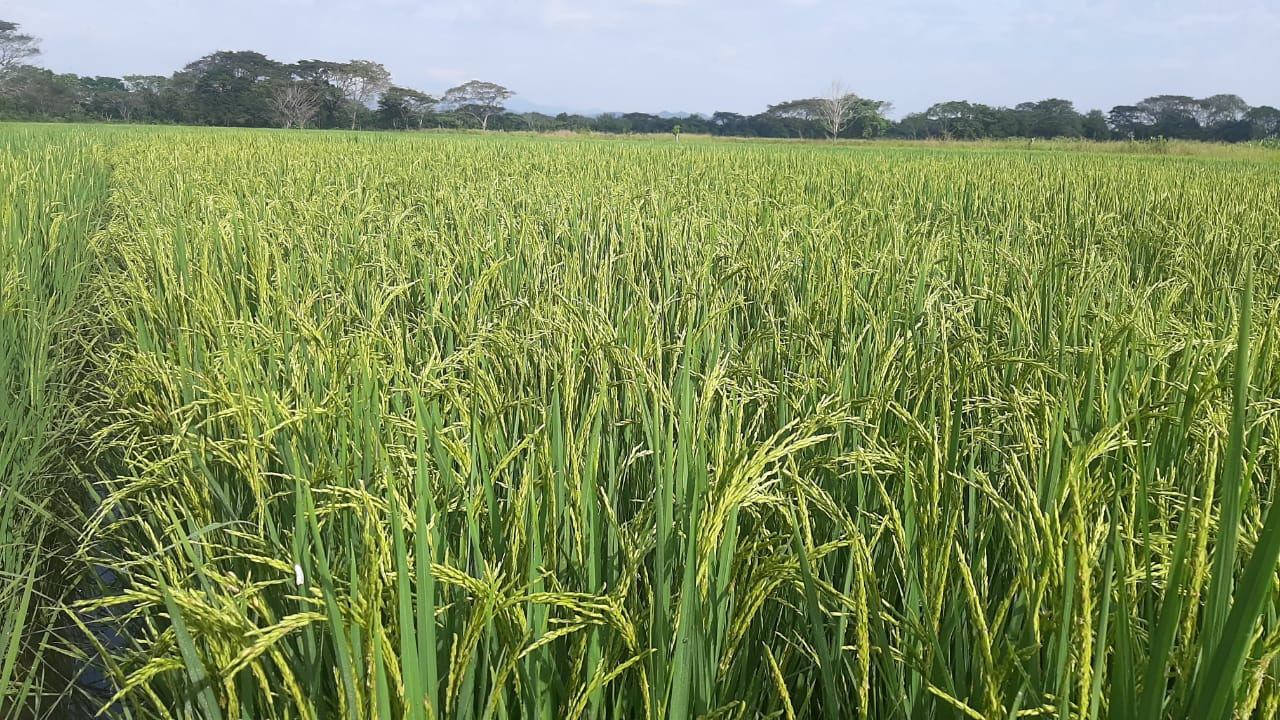
\includegraphics{AP009-9.jpeg}

\subcaption{\label{}Suprema FL en fase reproductiva}
\end{minipage}%
%
\begin{minipage}{0.50\linewidth}
Suprema FL\end{minipage}%

\end{figure}%

\subsubsection{\texorpdfstring{\textbf{Manejo del
riego}}{Manejo del riego}}\label{manejo-del-riego}

La variedad \textbf{SUPREMA} \textbf{\emph{FL}} no demanda el
establecimiento de láminas de agua por largos periodos de tiempo. Al
igual las demás variedades que se comercializan en la actualidad, puede
ser manejada con mojes en la fase vegetativa y solo durante las etapas
correspondiente a la fase reproductiva recomendamos que se establezca la
lámina para garantizar el normal desarrolla de de emergencia de
panículas, floración, grano lechoso y grano pastoso. Estas etapas son
críticas para definir un buen llenado y calidad de grano.

\subsubsection{\texorpdfstring{\textbf{Cosecha}}{Cosecha}}\label{cosecha}

\textbf{\emph{SUPREMA FL}} puede tolerar retrasos a la cosecha, siendo
una característica importante por los diferentes factores que pueden
interferir al momento de ejecutar la recolección del grano (lluvia,
logística de cosecha, accidentes de maquinaria entre otros).

Recomendamos que se revise periódicamente la calibración de la
cosechadora combinada para reducir las pérdidas que con frecuencia
suceden durante esta importante tarea.

Humedad del grano ideal para la recolección: entre 22\% y 20\%.Si tiene
preguntas o dudas sobre la información de manejo de la
\textbf{\emph{SUPREMA FL}}, no dude en consultarnos a los correos:

\begin{itemize}
\item
  \href{mailto:aproscello@gmail.com}{\nolinkurl{aproscello@gmail.com}}
\item
  \href{mailto:orlandoinvestiga@gmail.com}{\nolinkurl{orlandoinvestiga@gmail.com}}

  \ldots{} y con mucho gusto ampliaremos la información.
\end{itemize}

\begin{figure}

\begin{minipage}{0.50\linewidth}


\includegraphics[width=2.60417in,height=\textheight]{logo.png}

\subcaption{\label{}Rif: J-08507040-0}
\end{minipage}%
%
\begin{minipage}{0.50\linewidth}

\textbf{Ing. Yuraima Mendoza}

\emph{Fitomejoradora}

\textbf{Ing. Msc. Orlando Pérez}

\emph{Gerente de Tecnología y Desarrollo}

\end{minipage}%

\end{figure}%



\end{document}
